\documentclass[letterpaper, 11pt]{article}

\usepackage{lastpage, marginnote, siunitx, hyperref, amsmath, color, xcolor, graphicx}

%\definecolor{orange}{rgb}{1,0.5,0}

\def\UrlBreaks{\do\/\do-}

%\usepackage[hyphens]{url}

\usepackage{geometry}
\geometry{hscale=.6, vscale=.8, hmarginratio=2:1, vmarginratio=1:1, marginparwidth=.18\paperwidth, ignoremp}
%\geometry{marginparwidth=.1\paperwidth}

%\usepackage[T1]{fontenc}

\usepackage[explicit]{titlesec}
\titlespacing*{\section}{\dimexpr -\marginparsep-\marginparwidth}{*4}{*1}
\titleformat{\section}[runin]{\large\bfseries\titlerule[.5pt]\filright}{\makebox[1em][c]{\thesection}}{1em}{\parbox[t]{\dimexpr\marginparwidth-2em}{#1}\hskip\marginparsep\mbox{}}[\newline\vspace{-4ex}]

%\titlespacing*{\subsection}{\dimexpr -\marginparsep-\marginparwidth}{*4}{*1}
%\titleformat{\subsection}[runin]{\large\bfseries\titlerule[.5pt]\filright}{\makebox[1em][c]{\thesection}}{1em}{\parbox[t]{\dimexpr\marginparwidth-2em}{#1}\hskip\marginparsep\mbox{}}[\newline]

\usepackage{enumitem}
\newlist{steps}{enumerate}{1}
\setlist[steps]{label=Step \arabic*, font=\bfseries, leftmargin=-\marginparsep, itemindent=\marginparsep, align=right}

\usepackage{fancyhdr}
\pagestyle{fancy}
\fancyhf{}
\fancyhfoffset[lh,lf]{\dimexpr\marginparwidth+\marginparsep}
\fancyhf[lh]{UCD EEC 134}
\fancyhf[ch]{}
\fancyhf[rh]{}
%\fancyhf[lf]{left foot}
%\fancyhf[cf]{centre foot}
\fancyhf[rf]{Page \thepage /\pageref{LastPage}}
%\renewcommand{\footrulewidth}{.4pt}

%%%%%%%%%%%%%%%
%%%% Tikz definitions
%%%%%%%%%%%%%%%
%\tikzstyle{Uno}=[rectangle,fill=white,draw,line width=0.5mm]

%new commands
%display due date in red and link to the eec134-schedule.pdf document
\newcommand{\due}[1]{\href{https://github.com/ucdart/UCD-EEC134/blob/master/support/schedule/eec134-schedule.pdf}{\textcolor{red}{#1}}}

\graphicspath{{./figures/}}

\begin{document}

\title{Lab 6: Assembly of the Radar System}
\author{Instructor: Xiaoguang ``Leo'' Liu\\lxgliu@ucdavis.edu \\
	\small \href{http://creativecommons.org/licenses/by-sa/4.0/}{CC BY-SA 4.0}}
%\date{}
\date{Last updated: \today}

\maketitle


\section{Objectives}

\begin{enumerate}[itemsep=0.1ex]
	\item Understand basic radar system concepts. 
	
	\item Assemble and test a simple frequency modulated continuous wave (FMCW) radar using components built in the previous labs. 
	
	\item Understand radar signal processing techniques for velocity and range measurement. 
\end{enumerate}

%Be warned that this lab is a fairly aggressive one and it will take a lot of time for you and your group to finish all the reading, the pre-lab assignment, the actual lab, and the reports. It's a good idea to start early! And divide up tasks between group members wisely!
%\newpage
\section{Deliverables}
All items are to be submitted to the TA's email: eec134f2016@gmail.com.  

\vspace{0.5cm}

\begin{table}[h]
	\footnotesize
	\caption{Lab 6 Deliverables}
	\renewcommand{\arraystretch}{1.2}
	\begin{tabular}{|m{1in}|l|m{0.45in}|m{2in}|}
		\hline
		\textbf{Item} & \textbf{Due date} & \textbf{Format} & \textbf{File name format} \\
		\hline
		\hline
		Lab 6 report & \due{Dec.~8th, 2016} & pdf & ``lab-6-GroupName.pdf''\\
		\hline
	\end{tabular}
	\label{tab:deliverables}
\end{table}

\textbf{Notes:}
\begin{enumerate}
	\item All items are due by noon (12pm) of the due date. No late submissions are accepted. Don't even ask. 
	
	\item Please follow the file name format rigorously. Replace ``GroupName'' with your group's name and ``YourName'' with your name, first name first, last name last. 
\end{enumerate}

\newpage
\section{Prelab}

%\textbf{\Large Some critical concepts of radar systems}

\subsection{Radar range equation}
One of the fundamental parameters of a radar system is the maximum range $R_{max}$ at which the radar can detect an object. We can make some educated guesses on what $R_{max}$ may be related to. Obviously, if we send out more power, $R_{max}$ would increase. Alternatively, one could increase the gain of the antenna to increase the effective radiated power, that is, to concentrate the total radiated power towards the target direction (assuming we know where the target is). $R_{max}$ should also be target dependent. If the target is large and reflective, then it will reflect more power and is easier to detect. Correspondingly, the $R_{max}$ would be larger for such a target. Lastly, $R_{max}$ should depend on how sensitive the receiver is. 

Having done some qualitative analysis, let us now move on to some derivations. We already know from the previous lab that the radiated power density at a distance $R$ from a radiating antenna is 
\[
I_t = \frac{P_t G_t}{4\pi R^2},
\]
where $P_t$ is the transmitted power and $G_t$ is the gain of the transmitting antenna. 

Now the amount of power reflected from a target at a distance $R$ is not only dependent on $I_t$, but also on the target size, geometry, and material reflectivity. All of this can be captured into a single quantity, called the radar cross section (RCS) which has a dimension of area. Basically, a target with RCS of $\sigma$ looks like a perfect spherical reflector of cross-sectional area $\sigma$ and the reflected power is 
\[
P_{\sigma} = \frac{P_t G_t \sigma}{4\pi R^2}.
\]

Another assumption in the calculation and measurement of RCS is that the reflected power is assumed to be isotropic towards all directions. With this assumption in mind, the received power intensity at the location of the radar is
\[
I_r = \frac{P_t G_t \sigma}{4\pi R^2}\frac{1}{4\pi R^2}.
\]

The received power at the radar receiver is then
\[
P_r = \frac{P_t G_t \sigma}{4\pi R^2}\frac{A_{eff}}{4\pi R^2},
\]
where $A_{eff}$ is the effective aperture of the antenna and is related to the gain of the antenna by 
\[
G_r = \frac{4\pi A_{eff}}{\lambda^2}.
\]

Therefore, 
\[
P_r = \frac{P_t G_t \sigma}{\left( 4\pi R^2 \right)^2}\frac{G_r \lambda^2}{4\pi} =\frac{P_t G_t G_r \lambda^2 \sigma}{\left( 4\pi \right)^3 R^4}.
\]

Solving for the range $R$ we obtain the radar range equation

\begin{equation}
R = \sqrt[\uproot{16}4]{\frac{P_t G_t G_r \lambda^2 \sigma}{P_r \left( 4\pi \right)^3} }.
\end{equation}

The radar range equation gives a reasonable estimate of the maximum range of a radar at a given transmitter power and receiver sensitivity. 

\subsection{Pulsed radar}

Long range radar systems send and receive electromagnetic signals in \textit{pulsed} form (Fig.~\ref{fig:pulsedwaveform}). This allows the sensitive receiver to be turned off when the transmitter is transmitting. If we can measure the time $\tau$ that it takes for a pulse to travel to a target and return, then we can calculate the distance $d$ to the target as follows

\begin{equation}
d = \frac{c\tau}{2}
\end{equation}

The duration $t_p$ of the pulse is an important parameter in the design of pulsed radar systems. On the one hand, if the pulse duration is too short, then there is not enough average power in the signal for it to reach a long distance. On the other hand, if the pulse duration is too long, then the range resolution (resolution in the distance direction) of the radar degrades, because reflections from two closely spaced targets will smear with each other (Fig.~\ref{fig:pulserangeresolution}). The range resolution is given by 
\begin{equation}
\Delta R = \frac{ct_p}{2}.
\end{equation}

\begin{figure}[ht]
	\centering
	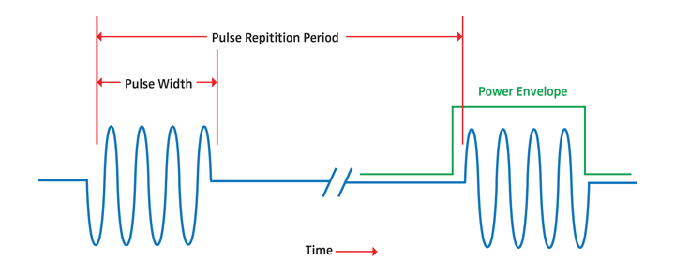
\includegraphics{pulsedwaveform}
	\caption{Pulsed radar waveform. \href{http://www.noisecom.com/resource-library/articles/characterizing-radar}{Source.}}
	\label{fig:pulsedwaveform}
\end{figure} 

\begin{figure}[ht]
	\centering
	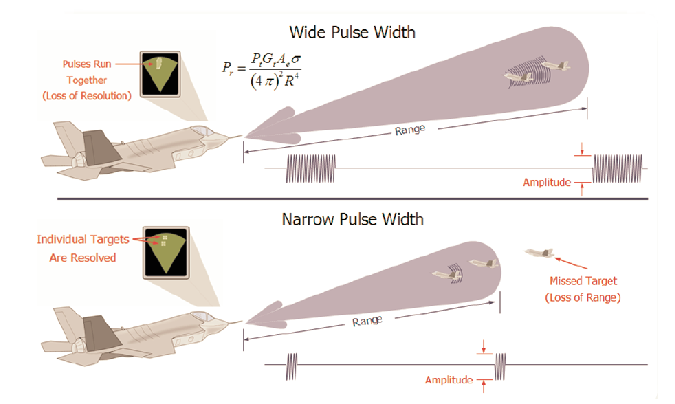
\includegraphics{pulserangeresolution}
	\caption{Range resolution of pulsed radar. \href{http://www.effectivebits.net/2011/08/radar-analysis-with-tektronix-mdo4104-6.html}{Source.}}
	\label{fig:pulserangeresolution}
\end{figure} 

\subsection{FMCW radar}
For short range applications, frequency modulated continuous wave (FMCW) radars are popular. This is the type of radar we are going to build in this lab.

In an FMCW radar, the transmitted signal is a continuous wave, i.e. on all the time, whose frequency changes with respect to time in a predefined pattern. The most common patterns are sawtooth and triangle ramps of the transmitted frequency (Fig.~\ref{fig:fmcwwaveform}). In practice, this is most commonly achieved by ramping up and down the control voltage of a VCO in the radar transmitter (Fig.\ref{fig:fmcwsystem}). 

After the radar signal leaves the transmitting antenna, its frequency will no longer change. Because the transmitter VCO keeps ramping up and down, when the reflected signal comes back to the radar receiver, it will see a different frequency coming out of the transmitter. The difference in frequency between the two signals can be extracted by a frequency mixer. This frequency difference is proportional to the round-trip delay of the radar signal to and from the target. By examining this frequency difference, the distance to the target can be calculated.

\begin{figure}[ht]
	\centering
	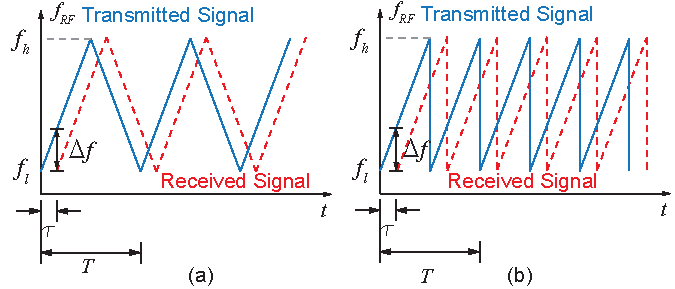
\includegraphics{fmcwwaveform}
	\caption{FMCW radar waveform.}
	\label{fig:fmcwwaveform}
\end{figure} 

\begin{figure}[ht]
	\centering
	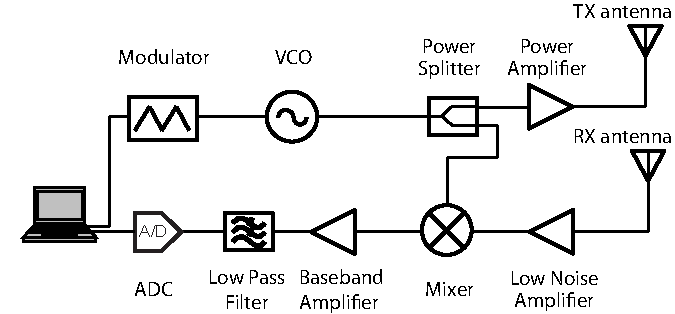
\includegraphics{fmcwsystem}
	\caption{Block diagram of a typical FMCW radar system.}
	\label{fig:fmcwsystem}
\end{figure} 

To see this more quantitatively, let's assume that we work with a triangle FMCW signal (Fig.~\ref{fig:fmcwwaveform}-a). The frequency ramp up and ramp down occur at a rate of $k$\,Hz/s and $-k$\,Hz/s. The time it takes for a transmitted signal to reach a remote target and come back is given by 
\[
\tau = \frac{2d}{c},
\]
where $d$ is the distance to the target. During this period, the frequency of the transmitter has changed by 
\[ 
\Delta f = k\tau = \frac{2kd}{c}.
\] 

Therefore
\[
d = \frac{c\Delta f}{2k}.
\]

The easiest way to measure $\Delta f$ would be to pass the received signal and the transmitted signal through a mixer. The frequency of the output of the mixer can then be determined by a frequency counter or digital signal processing. 

Because the frequency ramping is periodic, there can be ambiguities in the radar measurement. For example, if a target is far away enough, the returned signal may come back late enough to mix with the next ramp cycle and appear to be much closer than it really is. This ambiguity is determined by the period $T$ of the frequency ramp. The unambiguous range is given by 
\[
R_a = \frac{cT}{2}. 
\]

For FMCW radars, the range (distance along the main beam of the radar) resolution is determined by the bandwidth $BW = f_h - f_l$ of the frequency sweep as follows
\[
\Delta R = \frac{c}{2BW}. 
\]
Conceptually, this is consistent with a pulsed radar as the bandwidth of a pulse of duration $t_p$ is roughly $1/t_p$. 

Compared to a pulsed radar, the transmitter and receiver in a FMCW radar work at the same time. Because of a limited isolation between the transmitter and receiver, FMCW radars typically don't transmit high power and therefore are not used in long-range applications.

\subsection{Doppler Radar}

For some applications, we are only interested in the speed of remote targets. Speed can be measured by taking advantage of the Doppler effect. In a Doppler radar, the transmitted signal is fixed at one frequency. When the transmitted signal hits a moving target, the reflected signal is shifted in frequency according to the following relationship 
\[
f_r = \left( 1+\frac{v}{c} \right) f_0,
\] 
where $f_r$ is the frequency of the received signal, $v$ is the relative velocity of the target to the radar, and $f_0$ is the frequency of the transmitted signal. 

The system block diagram of a simple Doppler radar is essentially the same as Fig.~\ref{fig:fmcwsystem} except that the frequency is not modulated. 

\vspace{3ex}

% % % % % Pre-lab problems
%\reversemarginpar
%\marginnote{\textbf{Pre-lab Assignment}\\ Due: \due{Nov.~20th, 2015}}  Please answer the following questions:
%\begin{enumerate}[itemsep=0.1ex, label=\alph*)]
%	\item What are the advantages and disadvantages of using switch mode voltage regulator vs a linear voltage regulator?
%
%\end{enumerate}
%

\newpage
\section{Equipment \& \\Supplies}

\begin{itemize}[itemsep=0.5ex]
	\item 1 $\times$ bench power supply.
	\item 1 $\times$ bench oscilloscope.
	\item 1 $\times$ bench multimeter.
	\item 1 $\times$ wood board.
	\item 2 $\times$ TPI synthesizer;
	\item 1 $\times$ GSP-730 spectrum analyzer;
	\item 1 $\times$ USB battery pack;
	\item 4 $\times$ Male-male SMA-SMA connector. 
		\begin{figure}[h]
			\centering
			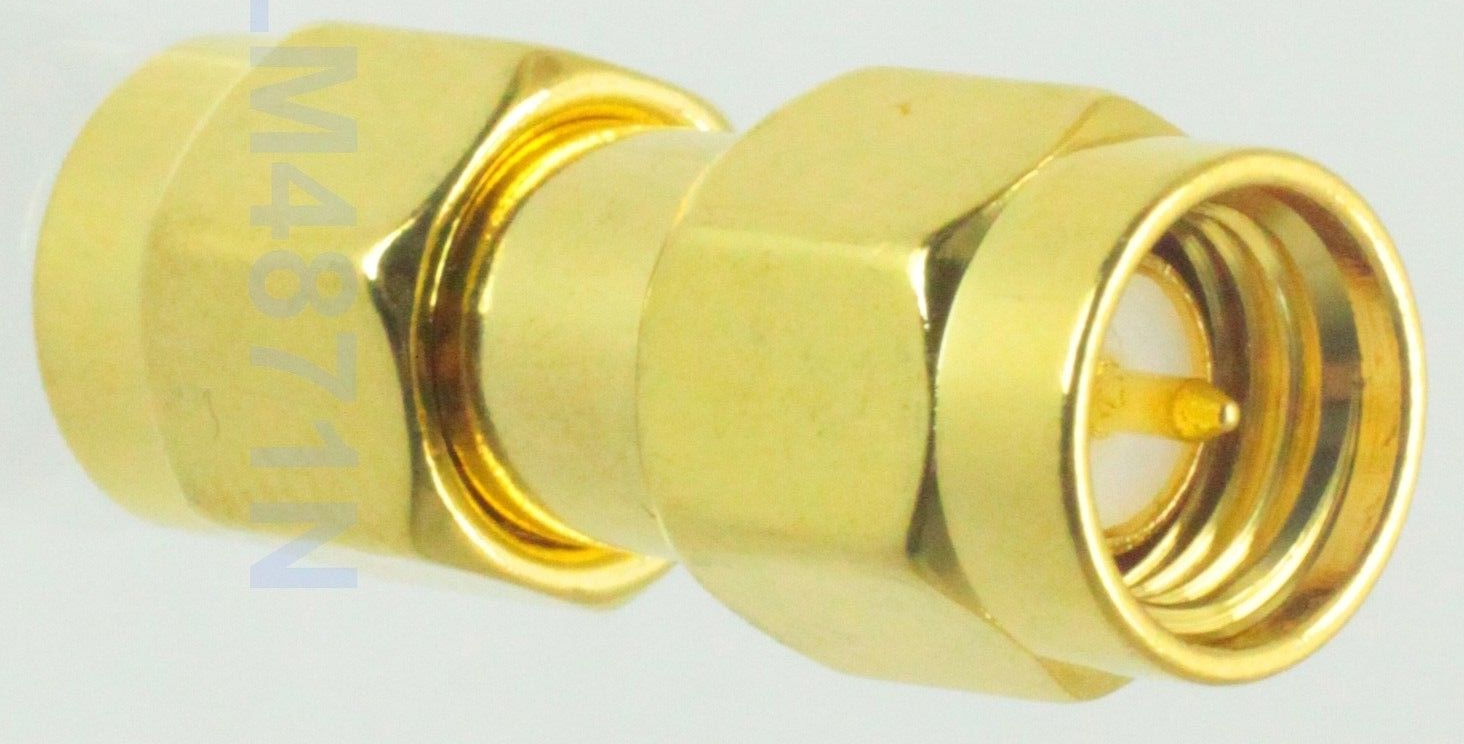
\includegraphics[width=2in]{sma-sma.png} 
			\caption{Male-male SMA-SMA adapter.}
			\label{fig:sma-sma}
		\end{figure}
	\item 1 $\times$ small screwdriver.
	\item 1 $\times$ custom made SMA-wire adapter.
	\item 1 $\times$ function generator from Lab 1.
	\item 1 $\times$ active low pass filter from Lab 1. 
	\item 1 $\times$ voltage regulator from Lab 1.
	\item 2 $\times$ Mini-Circuits ZX60-272LN-S+ RF amplifiers. 
	\item 1 $\times$ Mini-Circuits ZX95-2536C+ VCO. 
	\item 1 $\times$ Mini-Circuits VAT-3+ 3 dB attenuator. 
	\item 1 $\times$ Mini-Circuits ZX05-43LH-S+ mixer;
	\item 1 $\times$ Mini-Circuits ZX10-2-42+ power splitter. 
	\item 2 $\times$ coffee can antennas from Lab 5.
	\item Multiple \#2 and \#6 wood screws, provided by the TA. 
	\item 2 $\times$ L brackets. 
	\item 2 $\times$ 6'' and 2 $\times$ 12'' RF cables.
\end{itemize}

\newpage
\section{Procedures}

\subsection{System assembly}
In this lab, we will assemble the radar kit according to the block diagram in Fig.~\ref{fig:eec134system}. A wood board is going to be used as a platform to hold all the components of the system.

\begin{figure}[ht]
	\centering
	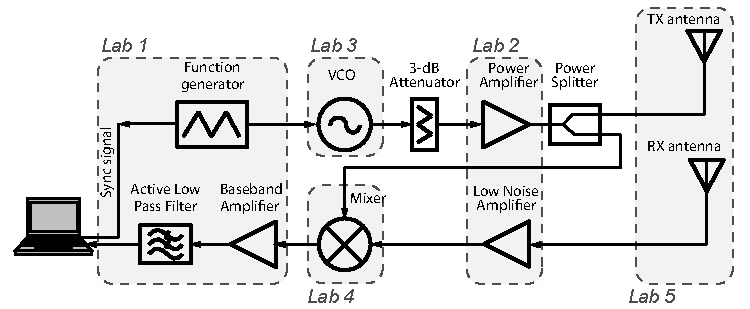
\includegraphics{eec134system} %TODO: add signal direction and points for pre-lab.
	\caption{Block diagram of the EEC 134 Quarter 1 FMCW radar system.}
	\label{fig:eec134system}
\end{figure}

\begin{enumerate}
	\item Connect the 3-dB attenuator with the output of the VCO. Connect the attenuator output to the input of the power amplifier (ZX60-272LN-S+) using an SMA-SMA adapter. 
	
	\item Connect the output of the power amplifier to the input of the power splitter (ZX10-2-42+) using an SMA-SMA adapter. 
	
	\item Remove the mounting bracket of the mixer (ZX05-43LH-S+) and the power splitter. This makes it easier to mount all the RF components on the wood board. Remember to put the two Phillips screws back to the mixer and the splitter. %TODO: need a picture here
	
	\item Connect one of the output ports of the power splitter to the mixer LO port using an SMA-SMA adapter.  
	
	\item Connect output of the low noise amplifier (LNA, the same ZX60-272LN-S+ amplifier) to the RF port of the mixer using an SMA-SMA adapter.
	
	\item Connect the output of the mixer to the SMA-wire adapter provided by the TA.
	
	\item Lay the above components down on to the wood board. Use \#2 wood screws to fix the microwave components on the wood board. Fig.~\ref{fig:rf-on-wood} shows an example; your board doesn't have to look the same. 
	
	\begin{figure}[h]
		\centering
		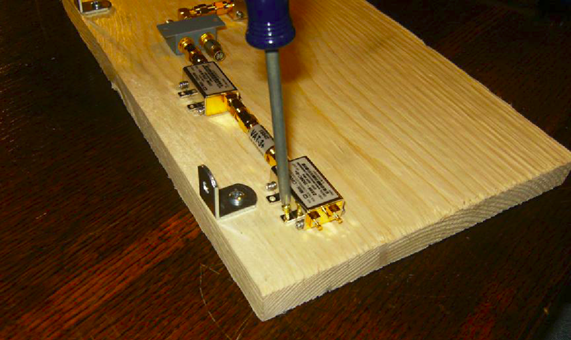
\includegraphics[width=3.5in]{rf-on-wood}
		\caption{An example layout of the RF components on the wood board.}
		\label{fig:rf-on-wood}
	\end{figure} 
	
	\item Mount your baseband circuits (battery, voltage regulator, modulator, LPF, etc) on the wood board, and connect them according to Fig.~\ref{fig:eec134system}. 
		\begin{enumerate}
			\item Adjust the function generator to output a triangle wave between 0.5\,V and 4.5\,V, with a ramp period of 40\,ms, i.e.~20\,ms for ramping up and 20\,ms for ramping down.
		\end{enumerate}
	
	\item Connect the power lines to all the RF components. Connect a ground wire to the ground terminal of one of the microwave modules and the baseband circuits. 
	
	\item Connect the audio cable to the breadboard circuit.
		\begin{enumerate}
			\item red = right channel is fed to the output of baseband amplifier + LPF
			\item white = left channel is fed to the SYNC output of the modulator
			\item shield is connected to the ground bus of the breadboard
		\end{enumerate} 

	Once connected, secure the audio cable to the wood board so that it doesn't get pulled easily from the circuit. 
		
	\item Mount the two coffee can antennas on to the wood board using two L bracket and \#6 wood screws. 
	
	\item Connect the receive antenna to the input of the LNA using an SMA-SMA coaxial cable. Connect the transmit antenna by connecting the unused output of the splitter to the second coffee can antenna using an SMA-SMA coaxial cable. The radar system is now complete! 
		\begin{enumerate}
			\item Include a picture of the final assembly in your lab report.
			
			\item Based on the system diagram, what is the output power that you expect to get at the output of the power amplifier? How much do you actually measure?
			
			\item Using your TPI synthesizer, feed a test RF signal of -30\,dBm at 2.4\,GHz to the input of your receiver (i.e. input of the LNA). Using a 10-dBm LO signal of 2.400001\,GHz, record the audio signal that you get at the output of the active low pass filter. What is the total voltage gain of your receiver? Gradually increase the input signal power, does the output increase linearly with the input? At what point does this linear relationship stop (P1dB point)?
		\end{enumerate}
	
\end{enumerate}

\subsection{Radar measurements}

In the preceding steps, you should have assembled your radar system, and tested your analog baseband and RF circuits. 

To test the basic radar functionality, you should connect the antennas and observe the audio signal output to get a crude idea whether the system is working. You can first try this by connecting the audio output to an oscilloscope. Place a reflective object, e.g. a metallic plate, in front of the radar and move it back and forth. You should observe a sinusoidal-like signal on the oscilloscope. When the reflector is closer to the antenna, the signal has a lower frequency (why?) and a larger magnitude (why?); when the reflector is farther away, the signal is weaker and of lower frequency. Obviously this doesn't guarantee that the system is working properly for all the following tests, but it at least gives you some confidence that the system is functioning as a radar.

The lab environment is not very friendly to characterizing your radar system because there are many strong reflectors and moving targets. Usually you will get much better results by testing the system outside in an open field. 

\subsubsection{Range measurement}

As explained in the prelab, frequency modulation is needed for the range measurement. 

\begin{enumerate}
	\item Connect the VTUNE pin of the VCO to the  function generator (Lab 1) output. Adjust the  function generator to output a triangle wave signal of 0.5\,V to 4.5\,V with a period of 40\,ms, i.e.~20\,ms for ramping up and 20\,ms for ramping down. Use as many voltage steps as you can. 
	
	\item Connect the radar output to the audio input of a computer. 
	
	\item Have one of your group mates slowly walk away or towards the radar. 
	
	\item Record the radar signal using Audacity (http://audacity.sourceforge.net/) and save it as a .wav file. The software is already installed on the lab computers.
	
	\item A Python script ``range\_wav.py'' is available at this link (\url{https://github.com/ucdart/UCD-EEC134/blob/master/labs/lab6/code/range_wav.py}) to process the recorded .wav file. An example .wav file named ``running\_outside\_20ms.wav'' can be analyzed for you to get an idea of the expected outcome. Fig.~\ref{fig:rti-cr} shows the range-time-intensity (RTI) plot of the data in ``running\_outside\_20ms.wav''. You can see two objects (people) walking away from and back to the radar. 
	
	\begin{figure}[h]
		\centering
		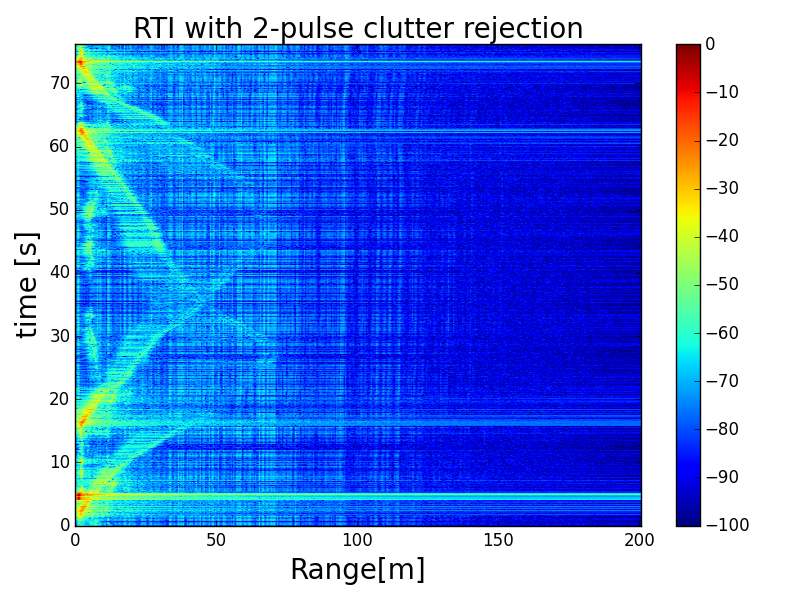
\includegraphics[width=3.5in]{rti-cr.png}
		\caption{Range-Time-Intensity (RTI) plot of the measurement data in ``running\_outside\_20ms.wav''.}
		\label{fig:rti-cr}
	\end{figure} 	
	
	
	To analyze your data, a few changes need to be made in the script.
	
		\begin{enumerate}
			\item Change the .wav file name to that of yours. By default, the .wav file needs to be in the same folder as the Python script.
			
			\item Change the ``Tp'' parameter to your ramp duration (20\,ms in this case)
			
			\item Change the ``fstart'' and ``fstop'' to the lowest and highest frequency of your sweep. You can get the values from the VCO datasheet. 
			
		\end{enumerate}
	\item Try to refine your measurement results and answer the following questions.
		\begin{enumerate}
			\item What is your measurement setup? What is the object that you measured? How is the environment like in terms of background reflection? You may include pictures for illustration. 
			
			\item Include your own plot of the range of a moving object. What is the typical range for the object under test? 
			
			\item Calculate the free-space range of our radar for a typical human with $\sigma$=1\,m$^2$. Compare with your test results.
			
			\item Explain how the code works. 
			
			\item What determines the cut-off frequency (15\,kHz in our system) of the low-pass filter? (Hint: What system parameters are impacted by changing the ramp time, say from 20\,ms to 1\,ms?)
						
			\item Any particular tricks or tips that you found helpful in improving the quality of the measurement? 
						
		\end{enumerate} 
	
	\item \textbf{(Optional):} You may find that the Teensy-based triangle wave generator introduces quite a bit of noise into the system. This problem can be alleviated by adding a low-pass filter after the DAC to filter out the high frequency noise. However, the cut-off frequency of the filter needs to be high enough to retain the triangle or sawtooth shape of the modulating waveform. 
	
	An alternative low-noise function generator can be built using all analog components. This application note (\url{https://www.maximintegrated.com/en/app-notes/index.mvp/id/4362}) gives one possible approach. 
	
	%	\begin{figure}[h]
	%		\centering
	%		\includegraphics{xr2206.png}
	%		\caption{.}
	%		\label{fig:xr2206}
	%	\end{figure}
	
\end{enumerate}

\subsubsection{Doppler measurement}
	\begin{enumerate}
		\item For Doppler (speed) measurement, we only need a single frequency CW output. Therefore, connect the VTUNE pin to a stable dc voltage, e.g.~5\,V. Make sure that the VCO output frequency at this voltage is within the operating range of your antenna. 
		
		\item You do not need to connect the SYNC signal. 
		
		\item  Point the radar to a moving target and record the .wav file. 
		
		\item A Python script ``doppler\_wav.m'' is available at \href{https://github.com/ucdart/UCD-EEC134/blob/master/labs/lab6/code/doppler_realtime_audio.py}{this link} to analyze the data. An example .wav file named ``highway\_doppler.wav'' can be analyzed for you to get an idea of the expected outcome. Fig.~\ref{fig:doppler} shows the velocity-time plot of the data in ``highway\_doppler.wav''. Fig.~\ref{fig:doppler} shows the velocity-time plot for the data in ``highway\_doppler.wav''. Each streak corresponds to a car passing by the radar which is mounted alongside a highway. As the car passes by the radar, it's relative speed to the direction of the radar antenna's main beam is very small but increases quickly as the car moves away from the radar. 
		
		\begin{figure}[h]
			\centering
			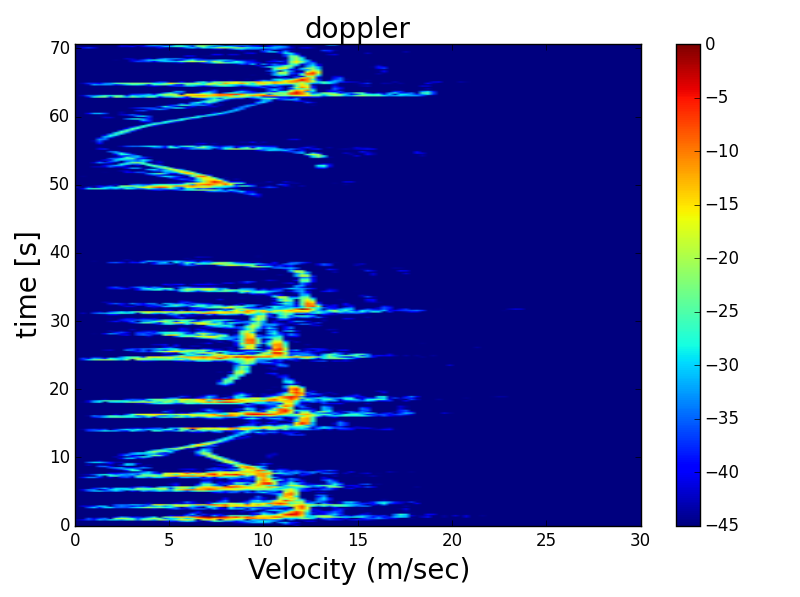
\includegraphics[width=3.5in]{doppler.png}
			\caption{Velocity-time plot for data in ``highway\_doppler.wav''.} 
			\label{fig:doppler}
		\end{figure} 	
		
		To analyze your data, the ``fc'' parameter in the script needs to be changed to the operating frequency of your radar system. This frequency can be determined by measurement. 
	
		A second Python script ``doppler\_realtime\_audio.py'' is also available in the ``code'' folder that will allow you to display the Doppler spectrum of the target in real time. The code is not guaranteed to work but should be easy to fix if it doesn't. 		
				
		\item Try to refine your measurement results and answer the following questions. 
			\begin{enumerate}
				\item Include your own plot of the speed of a moving object. 
				
				\item Measure the Doppler characteristics of an object or a machine that have exposed moving parts, such as a fan or a rotating bicycle wheel. 
				
				\item Explain how the code works. 

				\item Any particular tricks or tips that you found helpful in improving the quality of the measurement? 
			\end{enumerate}
		
	\end{enumerate}

\end{document}